\chapter{Results}
\label{cha:results}
\epigraph{
  This chapter will analyze the practical capabilities of the echo state
  network for anomaly detection in time series.  First we analyze the
  \emph{memory capacity} (MC) of the ESN and show how well the ESN can predict
  a scalar chaotic time series. A tradeoff between networks with large MC and
  good capability to predict non-linearities is discussed before moving on to
  two input images and sea surface height prediction.
}



\section{Short-term Memory}
\label{sec:short_term_memory}

The short-term memory capacity (\emph{MC}) of the internal state can be
estimated through the so-called coefficient of determination $R^2$  and a
simple experiment.  $R^2$ is the squared correlation coefficient. For two
variables $X$ and $Y$ it is defined by:
\begin{equation}
  \label{eq:detcoeff}
  R^2 = \text{detCoeff}(X, Y)
      = \frac{\text{cov}^2(X, Y)}{\sigma^2(X) \sigma^2(Y)}
\end{equation}

The network receives a random sequence $\mathbf{u}$ created from a uniform
distribution and is trained to extract the last $n$ inputs from the internal
state $\vt{x}$ with 20 units.  After training, the network extracts the last 40
time steps only from the last internal state
(Fig.~\ref{fig:random_timeseries_recovery}).
By creating $m$ sequences and collecting them in a matrix $U$
\begin{equation}
  U = \begin{bmatrix}
    u^{t=-n}_{0}  & \dots & u^{t=0}_{m} \\
    \vdots & \ddots & \vdots \\
    u^{t=-n}_{0}  & \dots & u^{t=0}_{m} 
  \end{bmatrix}
\end{equation}
and the reconstructions of the network in a corresponding matrix $Y$, the
coefficient of determination can be calculated for each time step by treating
the columns of $U$ and $Y$ as the variables $X$ and $Y$.
The memory capacity can then be estimated by:
\begin{equation}
  MC = \sum_{-n < i < 0} \text{detCoeff}(U_i, Y_i),
\end{equation}

The determination coefficient between extracted and targeted values is one if
they are equal and zero if there is no correlation between them at all.
\begin{figure}
  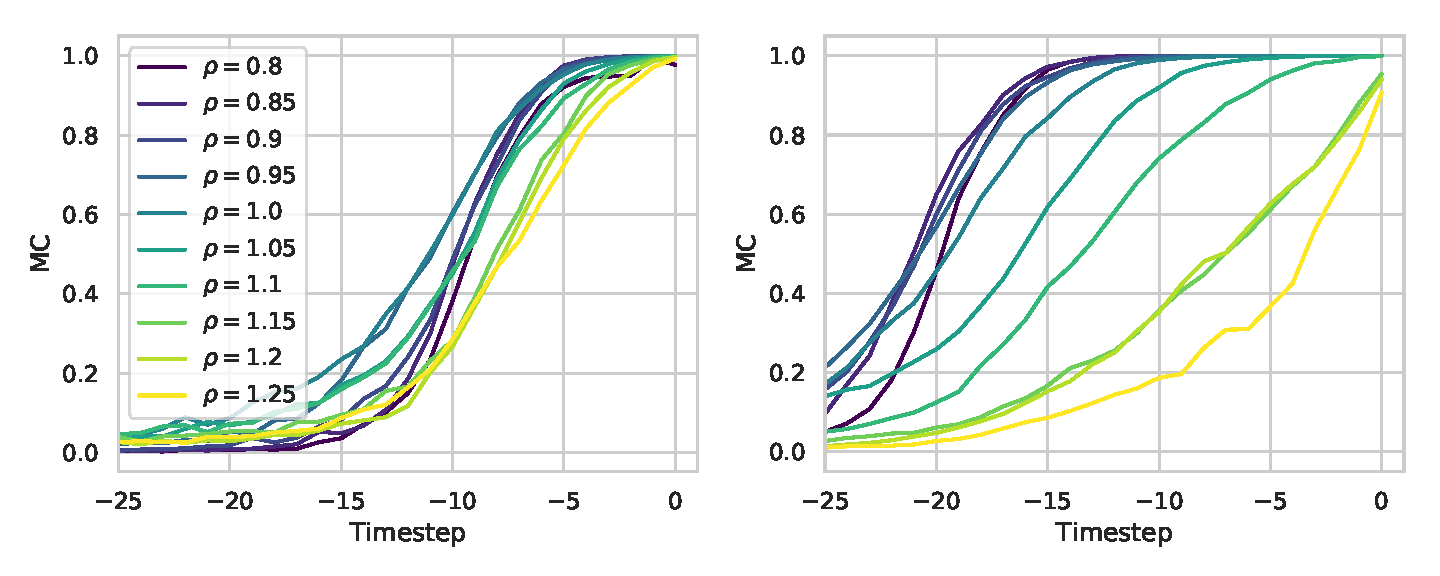
\includegraphics[width=\linewidth]{mc_seq.pdf}
  \caption{Determination coefficient over time for various spectral radii of
  the reservoir and two different learning algorithms. On the left the network
  was trained with GD and on the right with pseudo-inverse regression. The SGD
  trained network does not show a clear depedence on spectral radius, while in
  the LMS network it is clearly visible.}
  \label{fig:mc_seq}
\end{figure}

\begin{listing}
  \inputminted{json}{pseudocode/model_setups/memorize_setup.json}
  \label{lst:memorize_setup}
  \caption{ESN setup parameters for the memorization task. The \ttt{"False"}
    value of the Tikohnov regularization parameter $\beta$ means that the
    pseudo-inverse method was used. The spectral radius is varied from experiment
    to experiment.
  }
\end{listing}

To find the MC of the ESN it was trained with batches of $m=2000$ random
sequences.  Once with the Adam algorithm and once with the pseudo-inverse
method (which of course only need a single batch of random sequences to be
trained). After the training phase, another batch is fed to the network for
evaluation. An exemplary reconstruction is shown in
figure~\ref{fig:random_timeseries_recovery}.  It becomes evident that the most
recent time steps can be reconstructed almost perfectly and the memory of the
network becomes weaker further back in time.  With this setup one can try to
find the optimal spectral radius, which maximizes the memory capacity.  Both
plots in Fig.~\ref{fig:mc_seq} show the coefficient of determination over the
last 25 time steps at varying spectral radius $\rho$.  Interestingly, training
the ESN via a least mean squares approach (LMS, pseudo-inverse in this case)
seems to be much more efficient than training with Adam in this case.  In
addition, scaling $\rho$ has only a very small effect in the Adam-optimized
network, while it is clearly visible in the LMS ESN, but this is probably due
to the worse performance the SGD algorithm.  Figure~\ref{fig:mc_rho} suggests
that MC increases as $\rho$ approaches one and then quickly degenerates. This
is thoroughly investigated computationally in a paper by [\cite{farkavs2016}],
which in essence confirms the conjectures that were made before.

\begin{figure}
  \begin{minipage}[t]{.48\textwidth}
    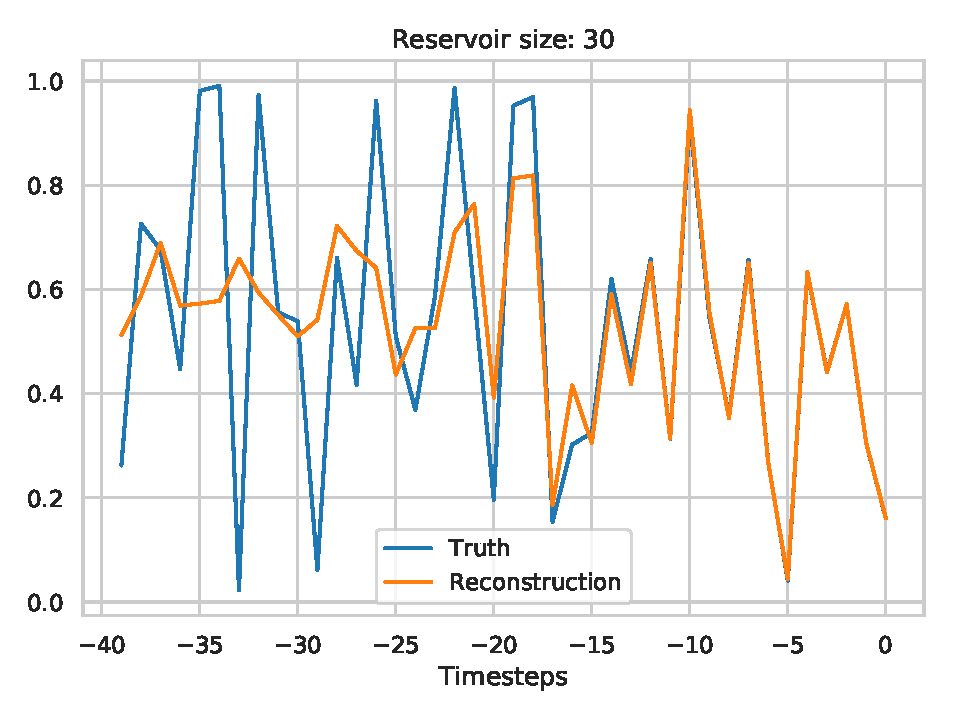
\includegraphics[width=\linewidth]{random_timeseries_recovery.pdf}
    \caption{
      True vs. reconstructed random time series. Most recent time step at $t=0$.
    }
    \label{fig:random_timeseries_recovery}
  \end{minipage}
  \hspace{.02\textwidth}
  \begin{minipage}[t]{.48\textwidth}
    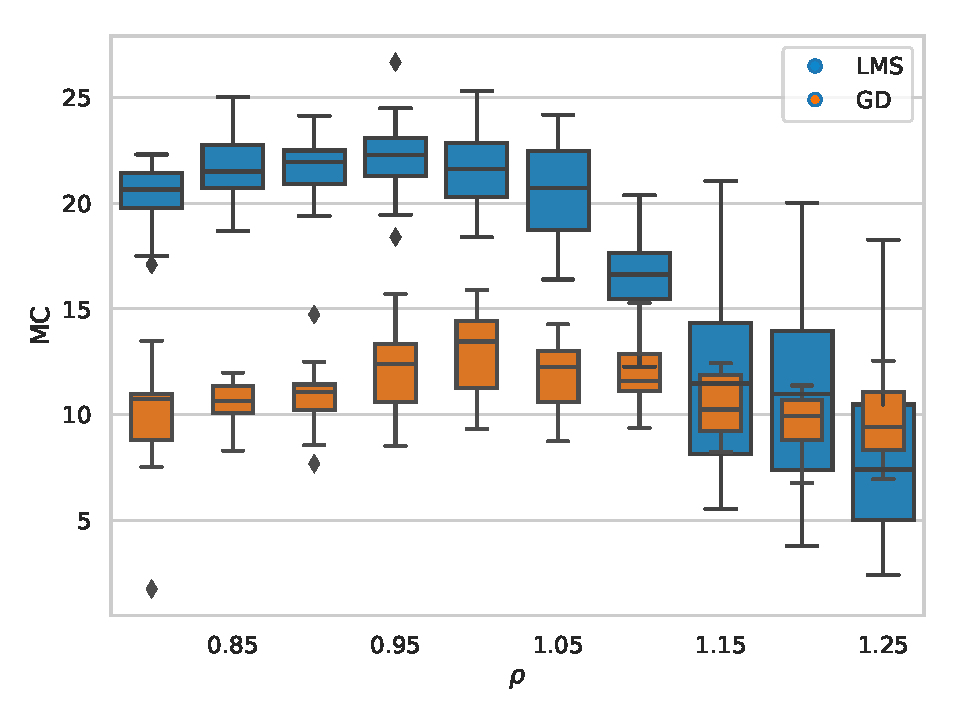
\includegraphics[width=\linewidth]{mc_rho.pdf}
    \caption{MC over spectral radius $\rho$ for the LMS and GD trained networks.}
    \label{fig:mc_rho}
  \end{minipage}
\end{figure}



\newpage
\section{Mackey-Glass System}%
\label{sec:res_mackey_glass_system}

\begin{figure}
  \centering
  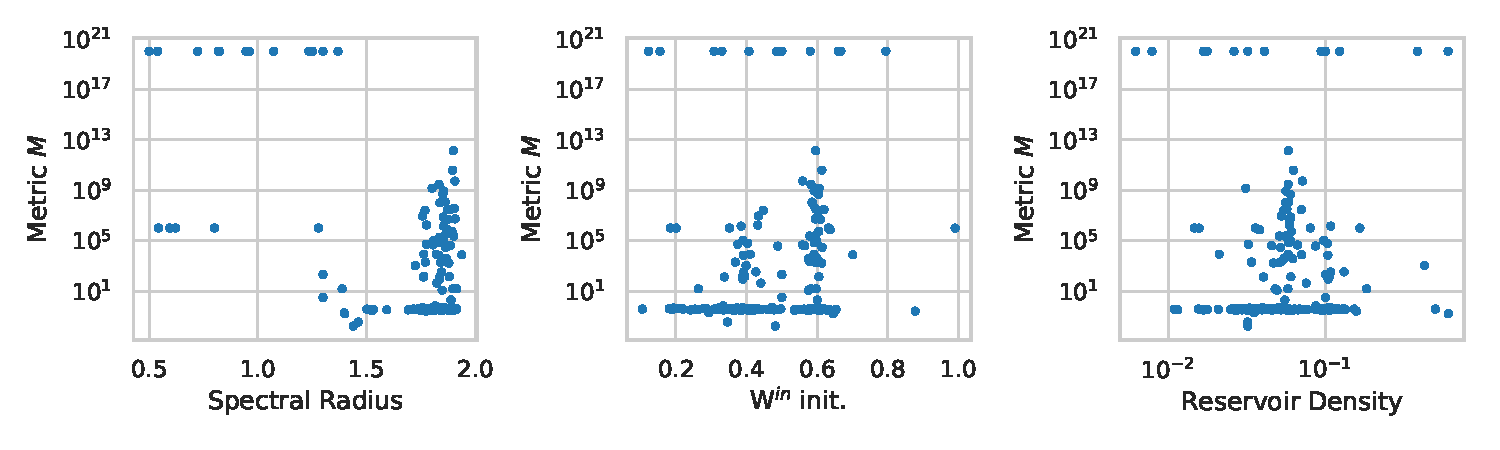
\includegraphics[width=\linewidth]{mackey_esn_ba_var_loss.pdf}
  \caption{Hyper-parameters over the squared error. The very large values
  are caused by diverging predictions that were clipped to a maximal
  $\mathrm{RMSE}=10^{20}$. The weight initialization and the sparsity
  parameters yield good performance in a certain range, the spectral radius
  only allows good performance for values larger than one.}
  \label{fig:mackey_esn_ba_var_loss}
\end{figure}


The first actual prediction task that will be solved by the ESN is the one of
the Mackey-Glass system that was described in
section~\ref{sec:mackey_glass_system}.  The reservoir is initialized with 500
units, which should be more than enough given that the period of the
considered time series is below 100 time steps, and that the ESN should have a
memory capacity slightly smaller than 500 steps.  The ESN is fed with a
sequence of length 2200, which creates the same number of internal states. To
avoid transients in the internal state, the first 200 steps are discarded. The
remaining 2000 internal states can be used to train the readout layer
$\wmatr{out}$ via the pseudo-inverse method. Three hyper-parameters (HP) remain
to be set: spectral radius, reservoir density, and input weight initialization
parameter, which are found with the help of Bayesian Optimization (BO).  For
this purpose, the package \ttt{scikit-optimize} was used to minimize the
RMSE
\begin{equation}
  \text{RMSE} = \frac{1}{N} \sum_{i=0}^N || d_i - y_i ||_2
\end{equation}
over several predictions.  The scikit algorithm needs an interval for every
parameter to form an HP space that it can sample from, which where chosen as
specified in table~\ref{tab:mackey_bo}. The resulting optimal HPs were obtained
over five BO runs.  Each BO run evaluated 100 trained ESNs at different points
in the HP space (Fig.~\ref{fig:mackey_esn_ba_var_loss}).  A surprising result
is that the optimal spectral radius is significantly larger than one.
In fact, the predicted signal just converges towards a value close to the mean
of the series if the spectral radius is close to one.
\begin{table}[h]
  \centering
  \rowcolors{2}{gray!25}{white}
  \begin{tabular}{|l c c c c|}
    \hline \rowcolor{gray!50}
    Parameter        & Best              & Min  & Max & Prior \\ \hline
    Spectral radius  & $1.40$   & 0.5  & 2.0 & uniform \\
    Weight init.     & $0.48$   & 0.1  & 1.0 & uniform \\
    Density          & $0.03$   & 0.01 & 1.0 & logarithmic \\
    \hline
  \end{tabular}
  \caption{Hyper-parameter results obtained via Bayesian Optimization}
  \label{tab:mackey_bo}
\end{table}

This is peculiar, as section~\ref{sec:short_term_memory} showed a spectral
radius close to one to be optimal for the memorization of sequences.  It
suggests that the crucial ingredient to predicting chaotic time series might
not only be a very good knowledge of the past, but something else. In fact this
is were the memory non-linearity tradeoff that was mentioned in
section~\ref{sub:short_term_memory} comes into play.  The more non-linear a
prediction task becomes the higher must the spectral radius of the reservoir be
to perform well. Unfortunately a large spectral radius degrades the MC of the
ESN. A mathematically sound framework for reasoning about the memory
non-linearity tradeoff is yet to be developed, but a rigorous computational
analysis of the problem is carried out in an article by [\cite{verstraeten2010}].
For the purpose of an anomaly detection it is enough that we found good
parameters for the prediction task. The quality of the predictions is depicted
in Fig.~\ref{fig:mackey1d_predictions}.
The predictive power of the ESN varies slightly over different parts of the
Mackey-Glass system. By randomly choosing different starting points in the
sequence and creating predictions for the next 500 frames, we can evaluate the
average error that the ESN makes at each frame.
Fig.~\ref{fig:mackey1d_predictions} shows the best and worst predictions in the
two upper plots and the average deviation of prediction and target in the
bottom.  An anomaly detection might be feasible within the first 100 frames, an
anomaly that is caught beyond that point might as well be caused by a degraded
prediction.\\

\begin{figure}
  \centering
  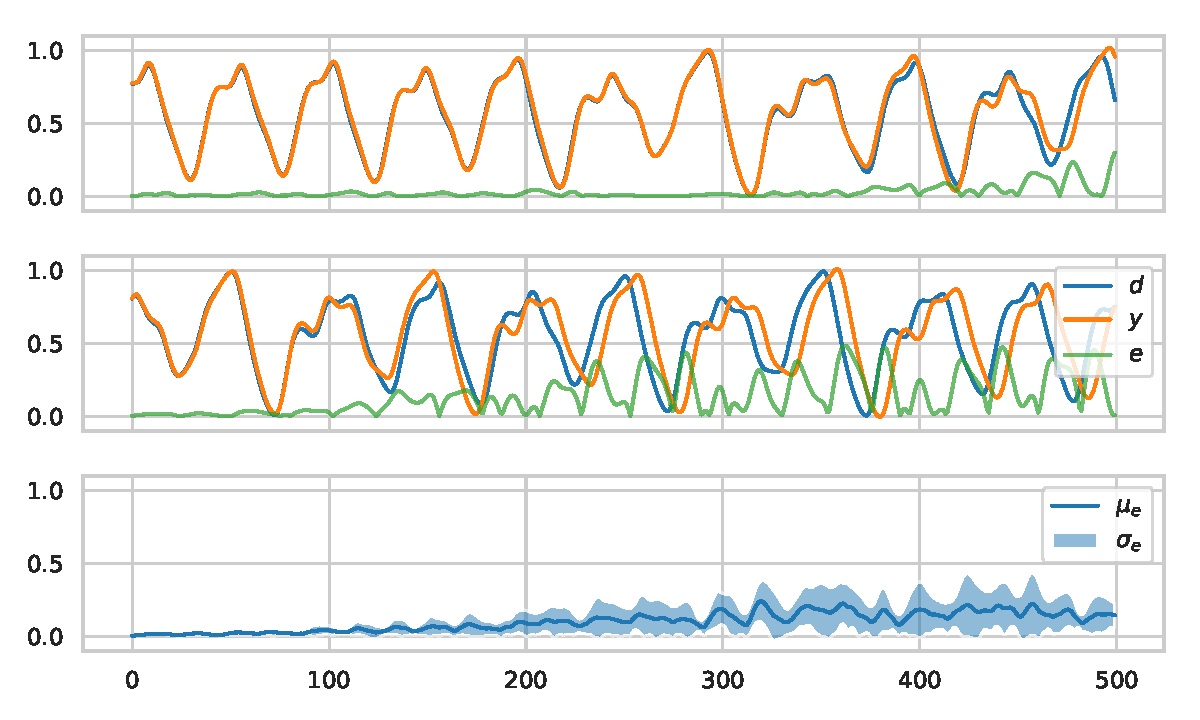
\includegraphics[width=\linewidth]{mackey1d_predictions.pdf}
  \caption{The best (top) and worst (middle) predictions from 20 randomly
    chosen starting points of the Mackey-Glass series. All predictions were
    made by an ESN with optimal hyper-parameters.  The target values $d$ are
    shown in blue, prediction $y$ in yellow, and the error $e = |d - y|$ in
    green.The plot in the bottom shows the variability of $e$ over different
    predictions.
  }
  \label{fig:mackey1d_predictions}
\end{figure}


At this point, \emph{finally}, all necessary parts to try and find artificially
introduced anomalies in the MG system are in place. The anomalies are created
by varying the parameter $\gamma$ of the MG Eq.~\ref{eq:mackey_glass}.  By
default it has a value of $\gamma = 0.1$.  Every 400 steps it is decreased by
an amount $\delta$ set back to its initial value after 50 steps. Depending on
the magnitude of $\delta$ this creates rather smooth looking anomalies. Easily
visual anomalies are created with a value of $\delta = 0.05$. To search the
outliers, the trained network receives a sliding window of 300 steps of the
anomalous sequence.  The predictions for the next $N_p = 50$ steps into the
future are collected and the \emph{mean prediction error} (MPE) is calculated
for every sequence that was fed to the ESN:
\begin{equation}
  \text{MPE} = \frac{1}{N_p} \sum_{t=1}^{N_p} | d_t - y_t |.
\end{equation}
The MPE is recorded for the whole dataset and the normality score $\Sigma$
(Eq.~\ref{eq:normality_score}) is computed with a large window size of 100
steps and a small window size of 5 steps..  The result is shown in
Fig.~\ref{fig:mackey_visible_anomalies}. With delight we can find that all
anomalies are easily caught.  To demonstrate the capabilities of the ESN to
efficiently find outliers in chaotic systems like the MG system,
Fig.~\ref{fig:mackey_anomalies} depicts how the algorithm performs on
anomalies that would, most probably, not be spotted by a human.

\begin{figure}
  \centering
  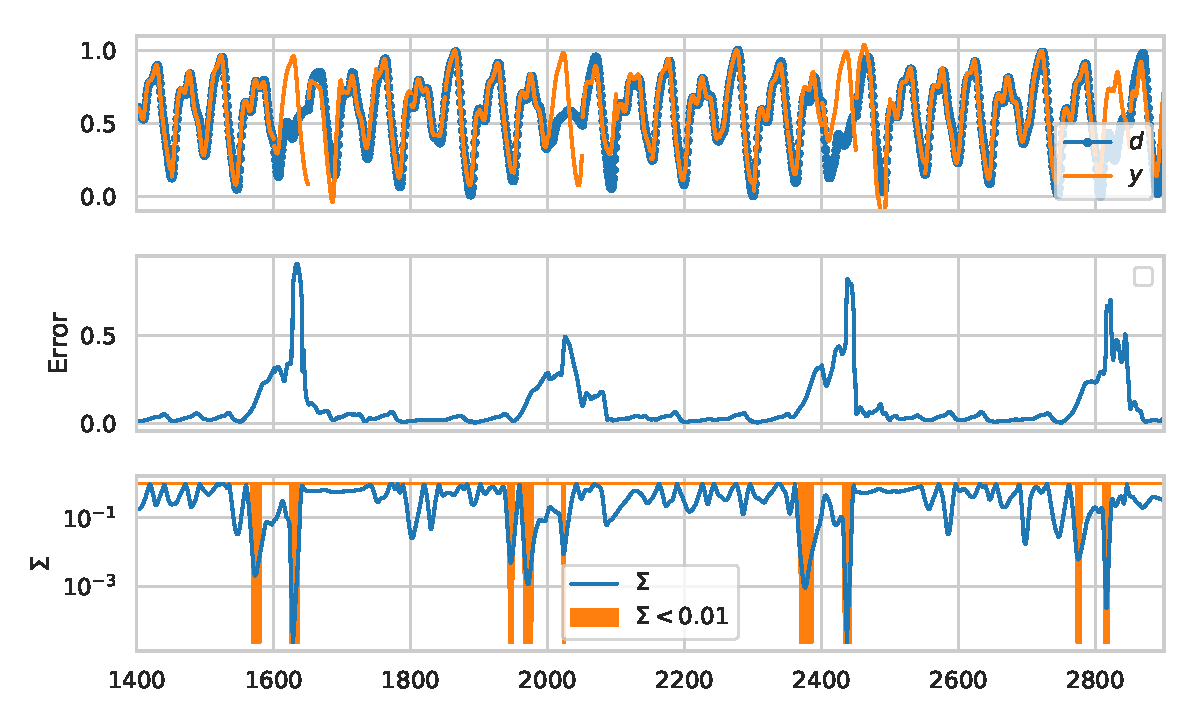
\includegraphics[width=\linewidth]{mackey_visible_anomalies.pdf}
  \caption{Mackey Glass system with artificially introduced anomalies at every
  400th step with $\delta=0.05$. The anomaly score catches the irregularly high error
  regions slightly too early, because the prediction error goes up as soon as the
  prediction window reaches into the anomalous regions.}
  \label{fig:mackey_visible_anomalies}
\end{figure}

\begin{figure}
  \centering
  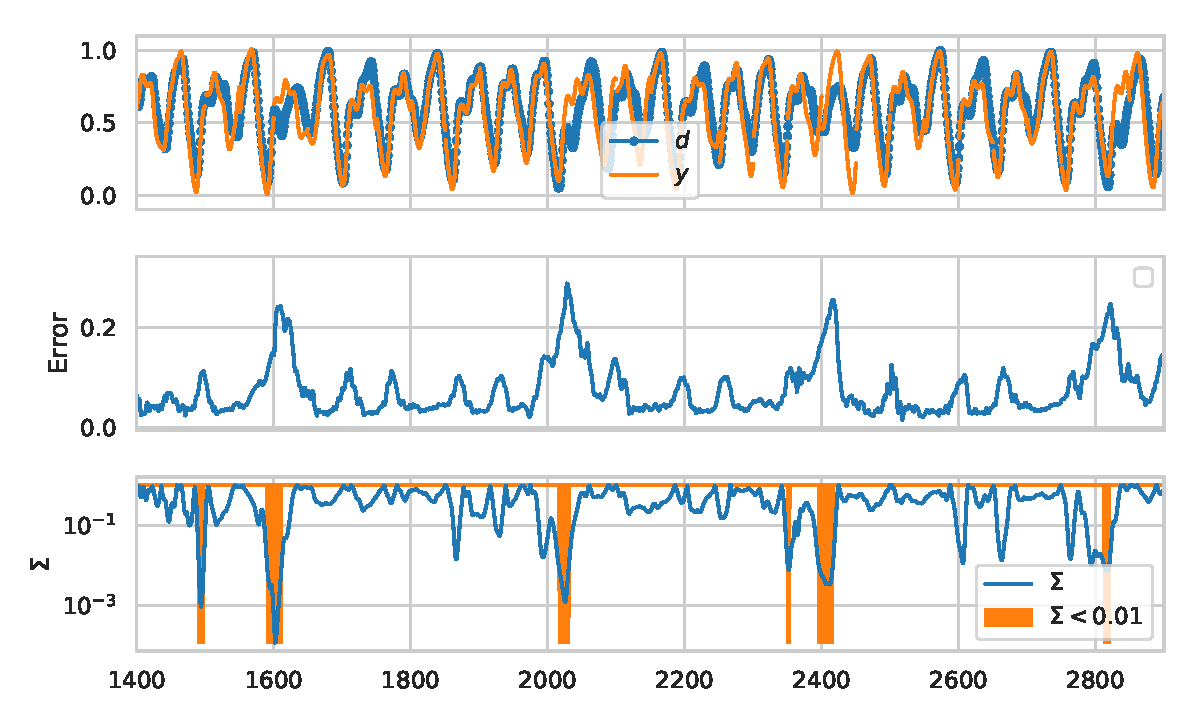
\includegraphics[width=\linewidth]{mackey_anomalies.pdf}
  \caption{Outliers that would have probably not been caught by humans. Created
  with $\delta = 0.03$. One false positive at $t=1500$.}
  \label{fig:mackey_anomalies}
\end{figure}

\begin{listing}
  \inputminted{json}{pseudocode/model_setups/mackey_setup.json}
  \label{lst:mackey_setup}
  \caption{ESN setup parameters for MG prediction.}
\end{listing}






\clearpage
\section{Dansgaard-Oeschger Events}%
\label{sec:res_dansgaard_oeschger_events}

The second dataset consisting of ice-core records that reach back 100k years
has two components. The $\delta^{18}$O sequence, which is directly connected to
surface temperature and the Ca$^{2+}$ series, that measures dust content and
shows similar patterns.  Both sequences lack a clear reappearing pattern, which
was clearly visible in the Mackey-Glass series, despite the chaotic nature of
the MG system. This makes a one time training over a part of the dataset that
contains most of variability impossible.  It should however still be possible
to project several dozen years ahead by moving to an online learning mode. In
the online mode, the output weights are recomputed with every new time slice
that is fed to the network.  The resulting short-term predictions $y$ are shown
in Fig.~\ref{fig:d18O_anomalies}.
\begin{listing}
  \inputminted{json}{pseudocode/model_setups/DO_setup.json}
  \label{lst:DO_setup}
  \caption{ESN setup parameters for DO event detection. The hyper-parameters were
  found via Bayesian Optimization.}
\end{listing}
They were achieved by training the ESN for 1500 input steps and predicting the
next 200 steps (the time step of the series is one year). Due to the very
irregular dataset the predictions are not very good, but at points where the
sequences change abruptly they deviate much more from the target values than
they do otherwise. This can be exploited to detect the DO events which are
located exactly at these abruptly changing points. Apart from the online weight
adaption, the procedure is the same as with the MG system. The score is calculated
from the MPE and thresholded, resulting in the detection of anomalies at the
yellow colored regions of Fig.~\ref{fig:d18O_anomalies}.
Abrupt changes after steady periods are easily detected by the algorithm.
DO events that lie close to each other tend to slip through. This is due to
the fact that the ESN learns from the previous DO events and as it is trained
on these anomalies, they are considered normal.
\begin{figure}
  \centering
  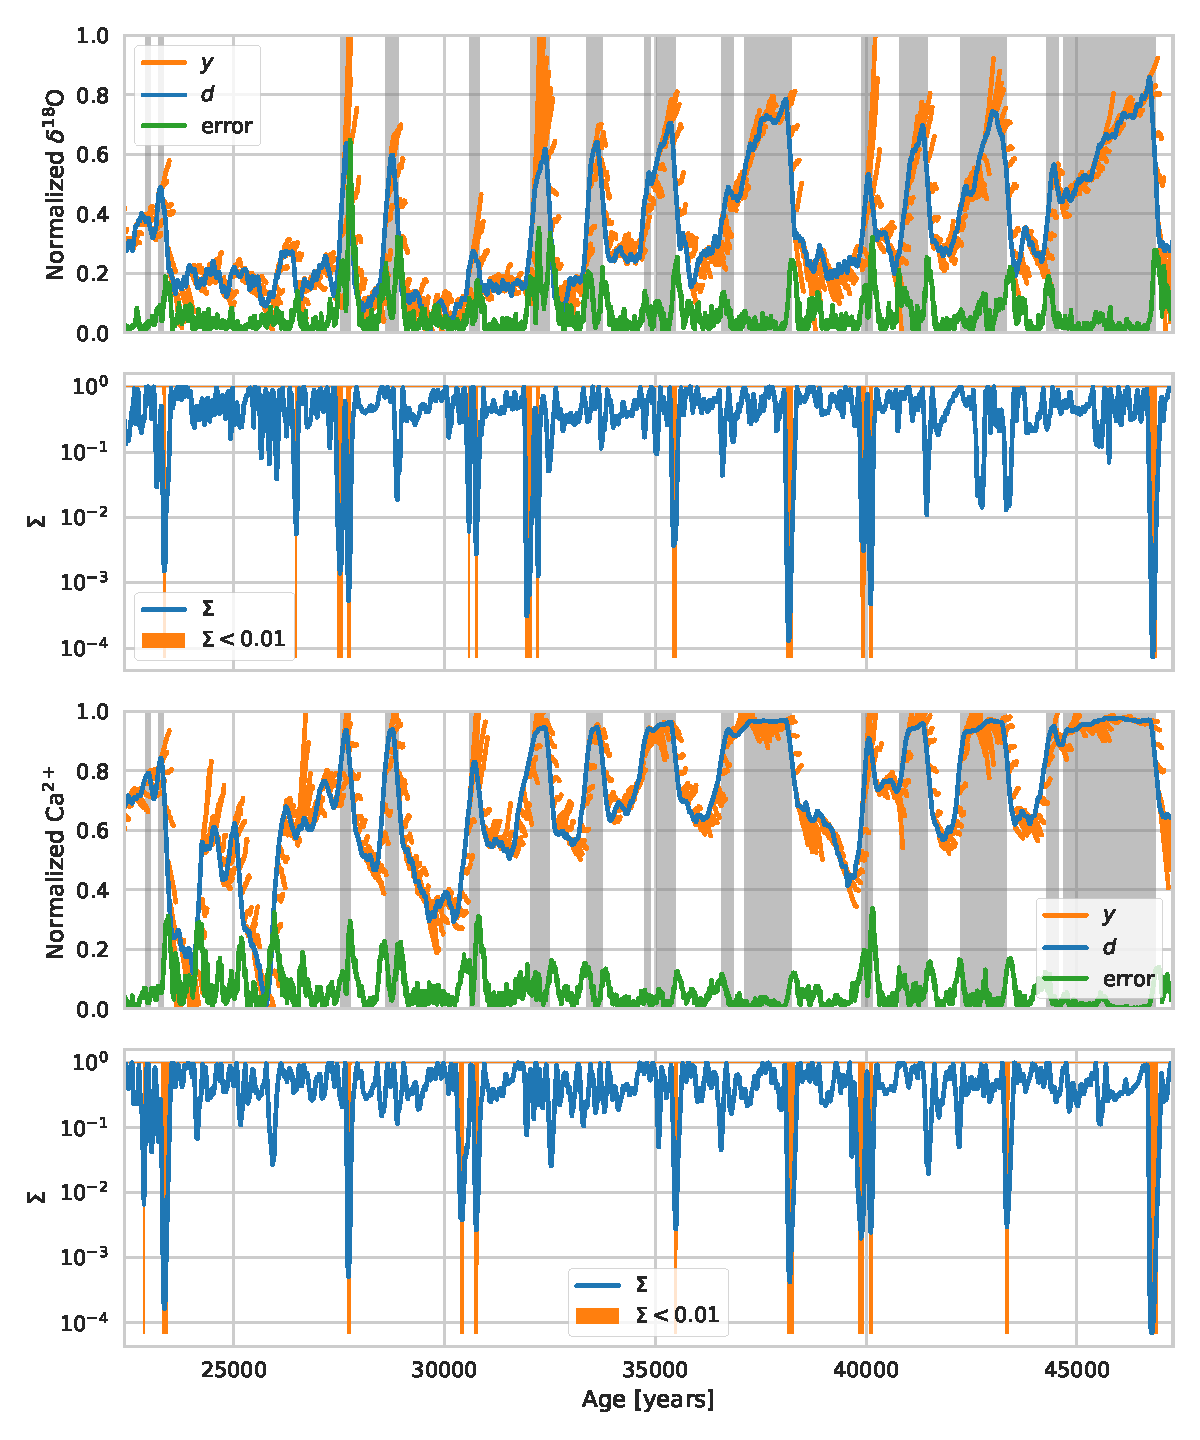
\includegraphics[width=\linewidth]{d18O_Ca2_anomalies.pdf}
  \caption{Detected anomalies in the DO dataset.}
  \label{fig:d18O_anomalies}
\end{figure}




\newpage
\section{Kuroshio}%
\label{sec:res_kuroshio}
\begin{figure}
  \begin{minipage}[b]{0.5\linewidth}
    \centering
    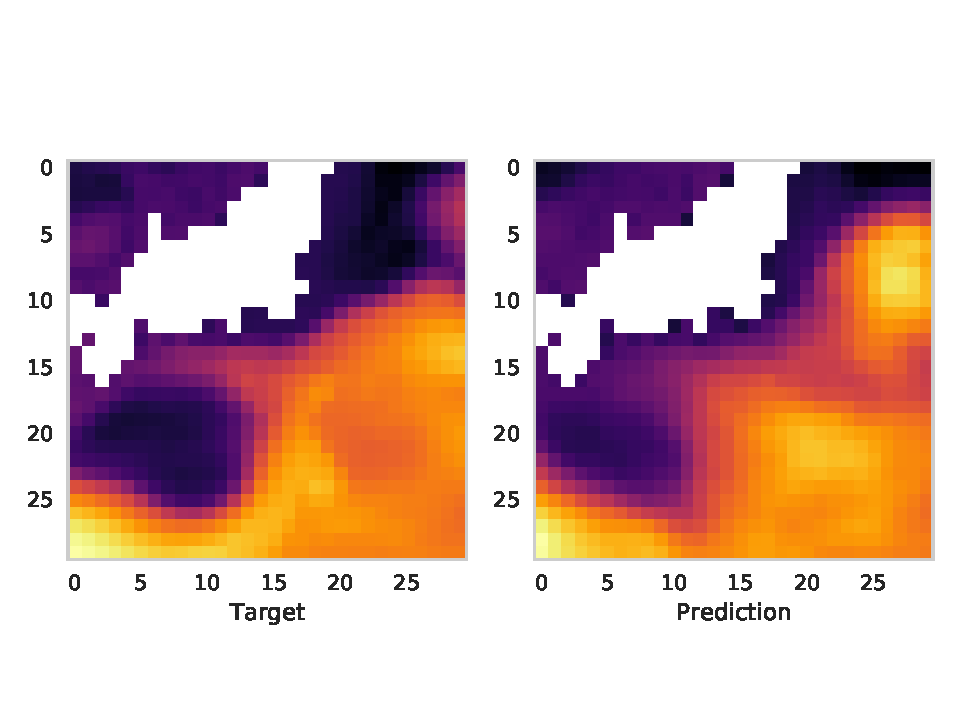
\includegraphics[width=.9\linewidth]{kuro_example_pred_stepidx200.pdf}
  \end{minipage}%% 
  \begin{minipage}[b]{0.5\linewidth}
    \centering
    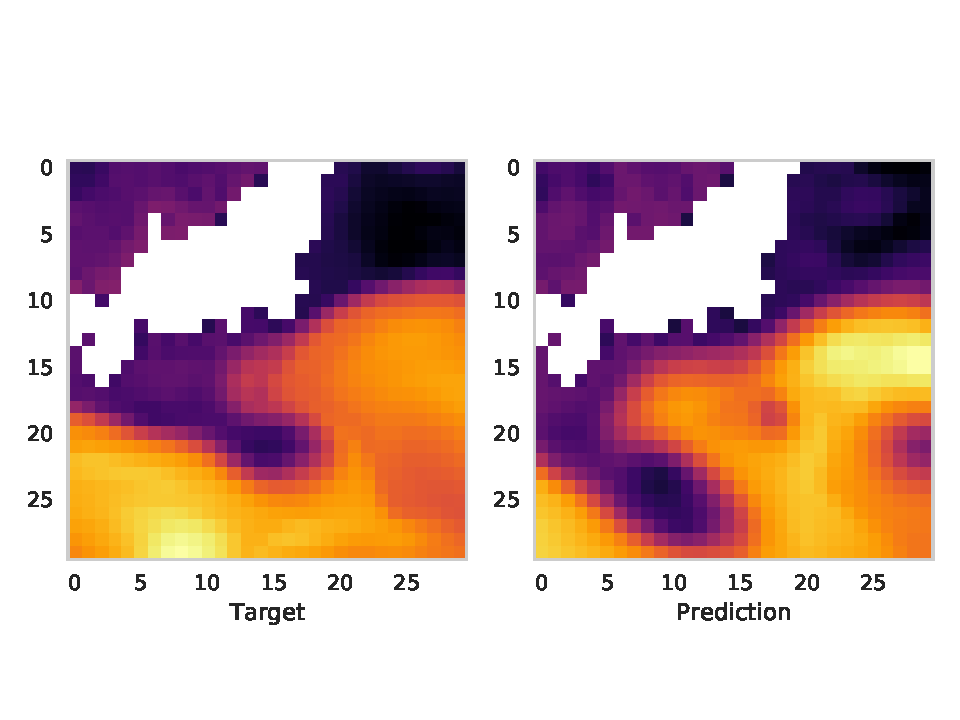
\includegraphics[width=.9\linewidth]{kuro_example_pred_stepidx470.pdf}
  \end{minipage} 
  \begin{minipage}[b]{0.5\linewidth}
    \centering
    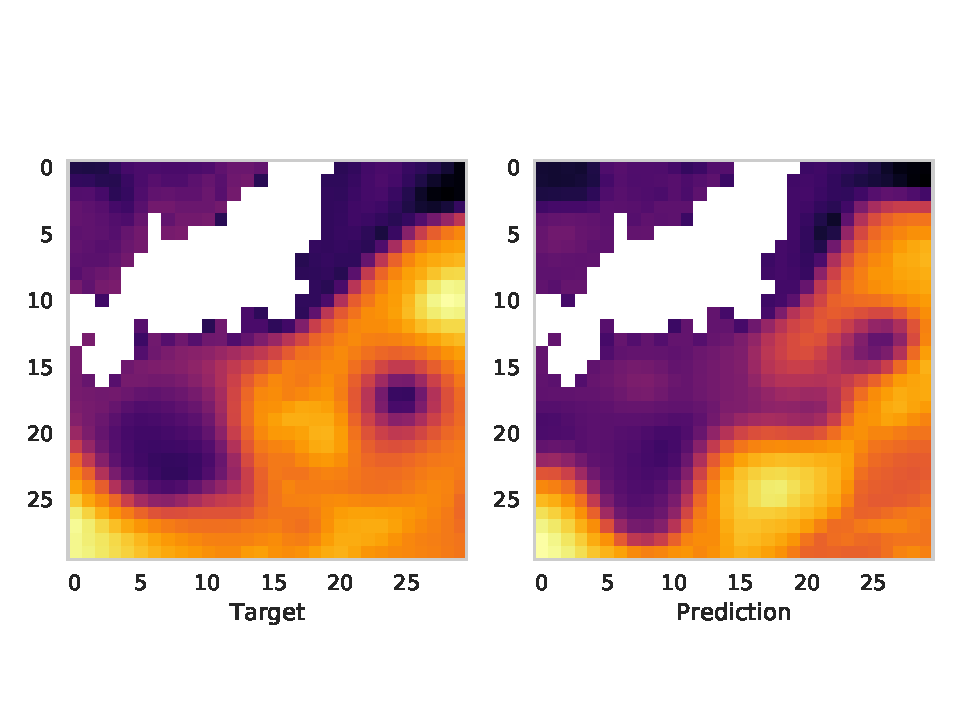
\includegraphics[width=.9\linewidth]{kuro_example_pred_stepidx0.pdf} 
  \end{minipage}%%
  \begin{minipage}[b]{0.5\linewidth}
    \centering
    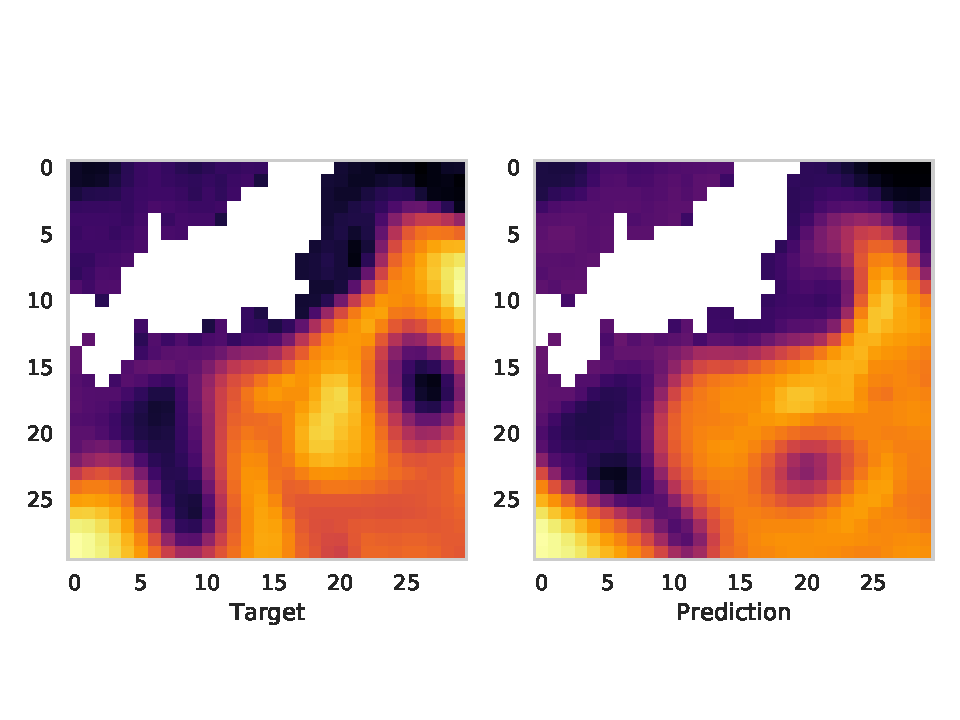
\includegraphics[width=.9\linewidth]{kuro_example_pred_stepidx100.pdf}
  \end{minipage} 
  \caption{Four exemplary predictions and corresponding desired outputs in the
    Kuroshio region. Shown is the 150th predicition frame out of 200.}
  \label{fig:kuro_pred_examples} 
\end{figure}


The prediction of the Kuroshio region involves significantly more data that
needs to be processed by the ESN. This means that the reservoir size has to
grow appropriately.  As a rule of thumb, the size of the internal state
$\vt{x}$ should be at least as big as the period of the dataset is long. The
most obvious period in climate simulations is typically the annual signal
which, in our case of 3-day means, is 122 steps long. To be able to remember
whole video sequences, this number should be multiplied by the number of pixels
in each frame to obtain the state size. Even if we consider raw inputs of 100 x 100
pixels and resample them to a size of 30 x 30, this would still result in a
state size greater than 100 000, which would result in a memory use of more
than 40 GB of the internal square reservoir matrix alone. This is clearly
unacceptable. Luckily, the pixels are highly correlated and we can hope that
the ESN is able to compress some of the information of the input images it
receives. Sizing the reservoir down to 10000 units and keeping it very sparse
will decrease the memory usage of the network to an acceptable amount of a few
hundred MB.

\begin{figure}[p]
  \centering
  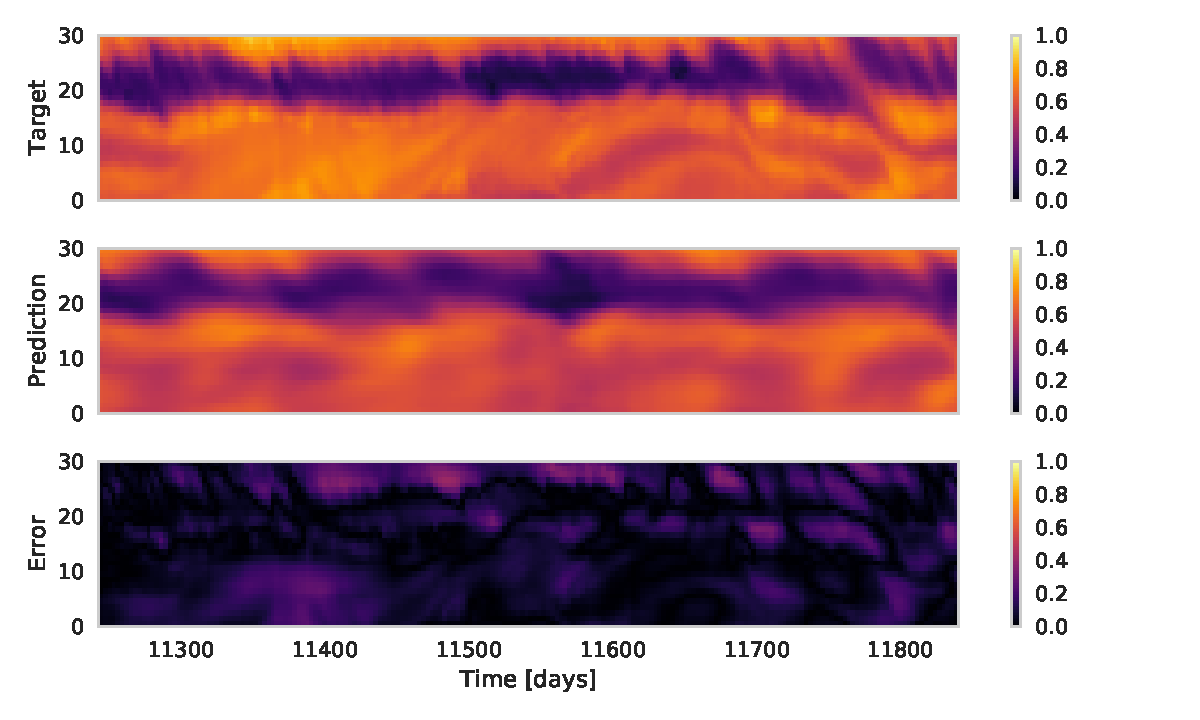
\includegraphics[width=1.1\linewidth]{kuro_pred_stepidx290}
  \caption{Exemplary prediction 200 steps into the future.}
  \label{fig:kuro_pred_stepidx290}
\end{figure}

\begin{figure}[p]
  \centering
  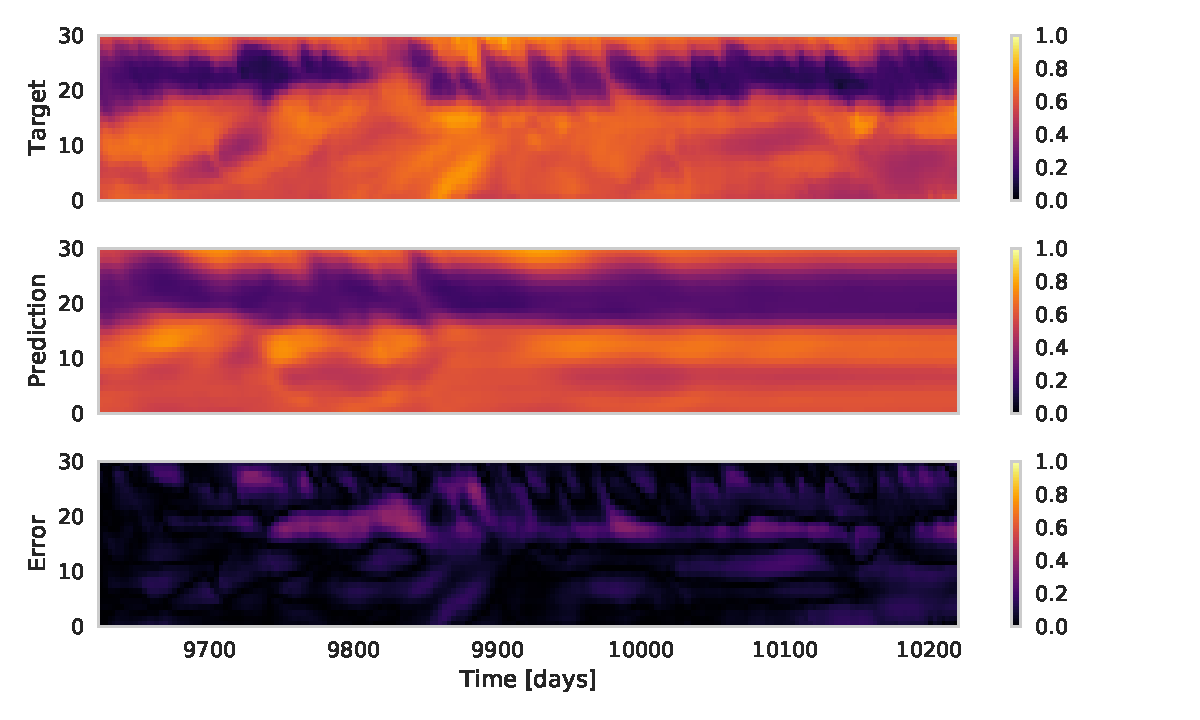
\includegraphics[width=1.1\linewidth]{kuro_pred_stepidx20}
  \caption{Another prediction example. Here it looks like the internal state of
  the ESN has reached a fixed point, so the prediction remains constant after
  day 10100.  This fixed point interestingly produces predictions that are very
  similar to the mean contracted state of the Kuroshio.}
  \label{fig:kuro_pred_stepidx20}
\end{figure}



Apart from using a sparsely represented ESN reservoir, the approach is again
the same as before.  The ESN receives 1300 input frames and predicts the next
200, which amounts to a prediction of roughly two years. Exemplary predictions
and the corresponding desired target outputs are shown in
Fig.~\ref{fig:kuro_pred_examples}. The figures ~\ref{fig:kuro_pred_stepidx290}
and ~\ref{fig:kuro_pred_stepidx20} show the 25th row of two more exemplary
target and prediction evolutions over time. The prediction error that is shown
is quite low for the predicted two years, but just to be sure only the first
year, meaning the first $N_p = 100$ frames, will be used for the subsequent
anomaly detection.

Fig.~\ref{fig:kuro_mean_pred} compares the target and prediction values for the
last prediction step ($N_p=100$) that is considered for the anomaly detection.
The error plot shows the MPE for each prediction. A large deviation of
prediction and target is visible around day 15500. The normality score (plotted
in a logarithmic color scale) that was calculated from the MPE sequence is very
low in this region as well. It seems to be a promising candidate for the
Kuroshio anomaly. By summing up all instances where the anomaly score $\Sigma <
0.01$ we can create a map of outliers. The result is shown in
Fig.~\ref{fig:kuro_anomaly_count}.  It shows a region with a lot of outliers
just where we expect them to be.  The similarity between the anomaly count and
the difference of elongated and contracted states is obvious and the result
will be regarded as a successful detection of the Kuroshio anomaly.

The second region of high anomaly counts is where the Kuroshio turns towards
the North Pacific basin. This anomaly is caused by a large unpredicted  eddy
that enters the analyzed area from the East. This anomalous region would
probably vanish if the analysis area is shifted eastward, away from Japan.
This would be the obvious next step of the outlier search, but unfortunately a
thorough analysis of the whole world is out of the scope of this work and will
remain as one path that a further studies of this problem could take.
\begin{figure}
  \centering
  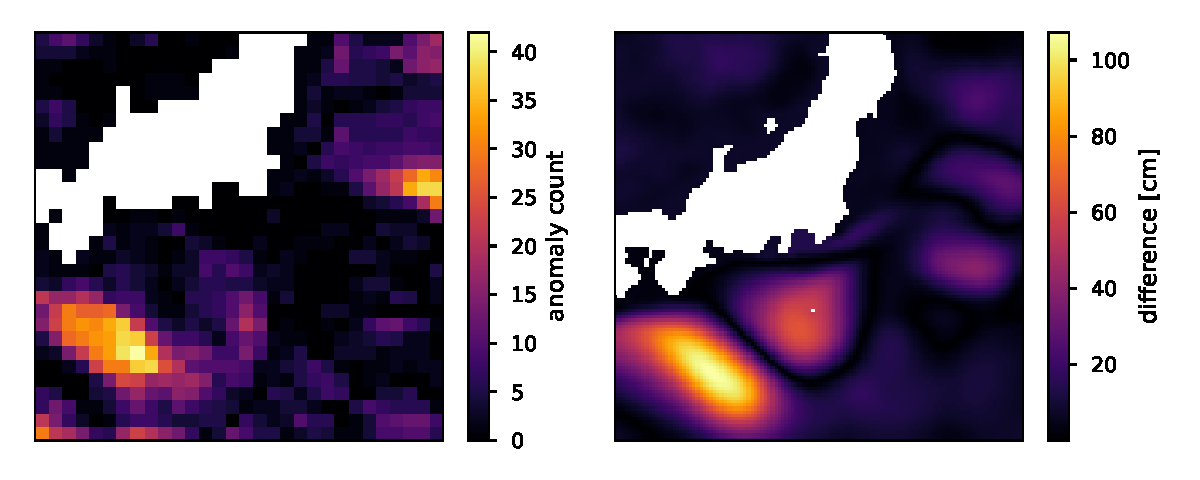
\includegraphics[width=\linewidth]{kuro_anomaly_count.pdf}
  \caption{Count of all pixels with a normality score that is lower than 0.01,
  compared to the assumed true form of the Kuroshio anomaly (obtained from the
  difference of its two states).}
  \label{fig:kuro_anomaly_count}
\end{figure}


\begin{figure}
  \centering
  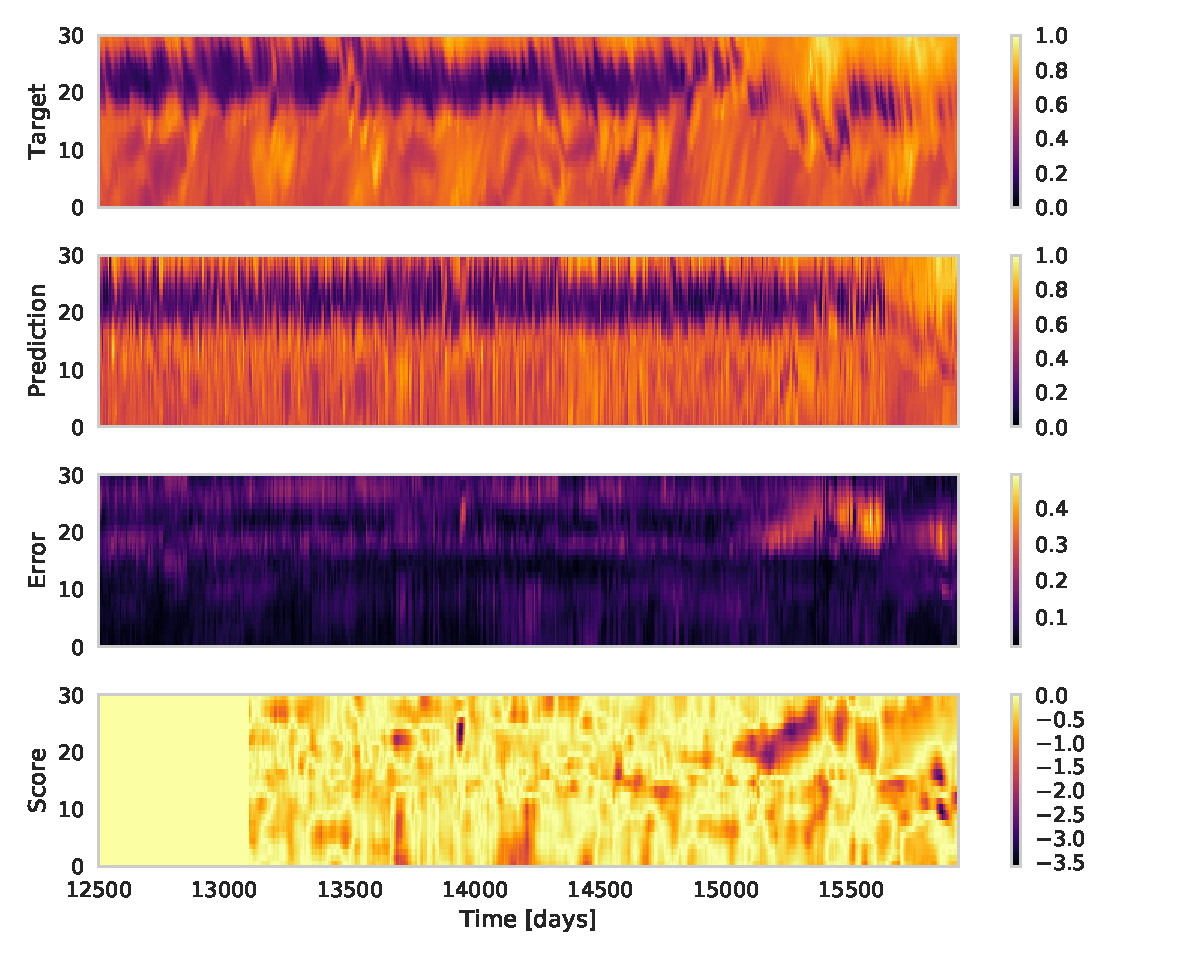
\includegraphics[width=1.1\linewidth]{kuro_mean_pred.pdf}
  \caption{The prediction plot shows the true values of one row of the SSH
    frames that were fed to the ESN.  In the target plot we can see the
    prediction that was made based on the internal state from 100 steps before.
    The error plot depicts the mean error of one prediction sequence and in the
    bottom we can see the resulting anomaly score on a logarithmic color scale.
  }
  \label{fig:kuro_mean_pred}
\end{figure}

\begin{listing}
  \inputminted{json}{pseudocode/model_setups/kuro_setup.json}
  \label{lst:kuro_setup}
  \caption{ESN setup parameters for Kuroshio anomaly detection. The Bayesian
  Optimization resulted a large range of parameters with similar performance as
  long as the spectral radius was larger than 1.3 and the weight initialization
  parameter larger than 0.8. The chosen hyper-parameters reflect the need for a
  sufficiently non-linear reservoir.}
\end{listing}
